\documentclass[11pt,a4paper]{article}
\usepackage[margin=1in]{geometry}
\usepackage[T1]{fontenc}
\usepackage{lmodern}
\usepackage{amsmath,amssymb,amsthm}
\usepackage{graphicx}
\usepackage{booktabs}
\usepackage[skip=6pt,font=small]{caption}
\usepackage{siunitx}
\usepackage[hidelinks]{hyperref}
\usepackage{cleveref}

\sisetup{exponent-product=\times, round-mode=none, group-minimum-digits=5}
\setlength{\textfloatsep}{12pt plus 2pt minus 4pt}
\setlength{\floatsep}{10pt plus 2pt minus 2pt}

\newtheorem{theorem}{Theorem}
\newtheorem{proposition}[theorem]{Proposition}
\newtheorem{lemma}[theorem]{Lemma}
\theoremstyle{definition}
\newtheorem{definition}[theorem]{Definition}
\theoremstyle{remark}
\newtheorem{remark}[theorem]{Remark}

% Auto-generated by scripts/export_macros.py from results/results.json. Do not edit.
\newcommand{\Kval}{\num{100}}
\newcommand{\rval}{\num{0.05}}
\newcommand{\sigmaval}{\num{0.25}}
\newcommand{\Tval}{\num{1}}
\newcommand{\Bone}{\num{80}}
\newcommand{\Btwo}{\num{130}}
\newcommand{\kval}{\num{1.6}}
\newcommand{\alphaval}{\num{-0.3}}
\newcommand{\betaval}{\num{-1.69}}
\newcommand{\taufinal}{\num{0.03125}}
\newcommand{\priceEighty}{\num{3.1415}}
\newcommand{\priceNinety}{\num{6.8698}}
\newcommand{\priceHundred}{\num{12.3360}}
\newcommand{\priceHundredTen}{\num{19.3051}}
\newcommand{\priceHundredTwenty}{\num{27.4063}}
\newcommand{\TableMethodsRows}{80 & \num{3.1415} & \num{3.1415} & \num{3.1398} & \num{3.1403} & \num{3.150} & [\num{3.133}, \num{3.168}] \\
90 & \num{6.8698} & \num{6.8698} & \num{6.8686} & \num{6.8675} & \num{6.888} & [\num{6.861}, \num{6.914}] \\
100 & \num{12.3360} & \num{12.3360} & \num{12.3351} & \num{12.3332} & \num{12.360} & [\num{12.324}, \num{12.396}] \\
110 & \num{19.3051} & \num{19.3051} & \num{19.3043} & \num{19.3026} & \num{19.335} & [\num{19.290}, \num{19.380}] \\
120 & \num{27.4063} & \num{27.4063} & \num{27.4054} & \num{27.4046} & \num{27.441} & [\num{27.387}, \num{27.494}] \\}
\newcommand{\errHeatKernel}{\num{2.5e-14}}
\newcommand{\errExplicit}{\num{0.0017}}
\newcommand{\errCN}{\num{0.0028}}
\newcommand{\errMC}{\num{0.034}}
\newcommand{\mcCoverCount}{5}
\newcommand{\mcSeMax}{\num{0.027}}
\newcommand{\fdDx}{\num{0.0125}}
\newcommand{\fdLam}{\num{0.4}}
\newcommand{\cnSteps}{\num{400}}
\newcommand{\mcPaths}{\num{1e6}}
\newcommand{\parityGap}{\num{5.7e-14}}
\newcommand{\stabDx}{\num{0.0125}}
\newcommand{\stabErrThirty}{\num{0.0016}}
\newcommand{\stabErrForty}{\num{0.0018}}
\newcommand{\stabErrHalf}{\num{0.0066}}
\newcommand{\stabErrFiftyTwo}{\num{2.2e10}}
\newcommand{\stabErrFiftyFive}{\num{2.2e26}}
\newcommand{\stabErrSixty}{\num{5.7e46}}
\newcommand{\TableStabilityRows}{0.3 & \num{0.2999} & 667 & \num{1} & \num{0.0016} \\
0.4 & \num{0.4000} & 500 & \num{1} & \num{0.0018} \\
0.5 & \num{0.5000} & 400 & \num{1} & \num{0.0066} \\
0.52 & \num{0.5195} & 385 & \num{1.08} & \num{2.2e10} \\
0.55 & \num{0.5495} & 364 & \num{1.2} & \num{2.2e26} \\
0.6 & \num{0.6006} & 333 & \num{1.4} & \num{5.7e46} \\}
\newcommand{\convOrderMax}{2.00}
\newcommand{\convOrderK}{2.00}
\newcommand{\convLocalMin}{2.000}
\newcommand{\convLocalMax}{2.002}
\newcommand{\TableConvergenceRows}{\num{0.025} & 125 & \num{0.00741} & \num{0.0035} \\
\num{0.0125} & 500 & \num{0.00185} & \num{8.79e-4} \\
\num{0.00625} & 2000 & \num{4.62e-4} & \num{2.20e-4} \\
\num{0.003125} & 8000 & \num{1.16e-4} & \num{5.50e-5} \\
\num{0.0015625} & 32000 & \num{2.89e-5} & \num{1.38e-5} \\}
\newcommand{\convErrFinest}{\num{2.9e-5}}
\newcommand{\convOrderOff}{2.00}
\newcommand{\convLocalOffMin}{2.00}
\newcommand{\convLocalOffMax}{2.00}
\newcommand{\convErrOffFinest}{\num{2.7e-5}}
\newcommand{\barA}{\num{-0.2231}}
\newcommand{\barB}{\num{0.2624}}
\newcommand{\barEll}{\num{0.4855}}
\newcommand{\barDiffMax}{\num{1.1e-5}}
\newcommand{\TableBarrierRows}{85 & \num{0.7610} & \num{4.7841} \\
90 & \num{1.3657} & \num{6.8698} \\
100 & \num{1.9621} & \num{12.3360} \\
110 & \num{1.7492} & \num{19.3051} \\
120 & \num{0.9755} & \num{27.4063} \\
125 & \num{0.4911} & \num{31.7656} \\}
\newcommand{\barPriceHundred}{\num{1.9621}}
\newcommand{\termsShortest}{51}
\newcommand{\termsLongest}{2}
\newcommand{\termsShortestDays}{1}
\newcommand{\termsPredShortest}{51}
\newcommand{\termsPredLongest}{2.7}
\newcommand{\nnPlainRmseTwenty}{\num{0.78}}
\newcommand{\nnPinnRmseTwenty}{\num{0.021}}
\newcommand{\nnPlainResTwenty}{\num{0.033}}
\newcommand{\nnPinnResTwenty}{\num{6.6e-4}}
\newcommand{\nnRmseRatioTwenty}{37}
\newcommand{\nnResRatioTwenty}{50}
\newcommand{\nnPinnSecondsTwenty}{111}
\newcommand{\nnPlainRmseFifty}{\num{0.31}}
\newcommand{\nnPinnRmseFifty}{\num{0.028}}
\newcommand{\nnPlainResFifty}{\num{0.017}}
\newcommand{\nnPinnResFifty}{\num{7.4e-4}}
\newcommand{\nnRmseRatioFifty}{11}
\newcommand{\nnResRatioFifty}{22}
\newcommand{\nnPinnSecondsFifty}{102}
\newcommand{\nnPlainRmseTwoHundred}{\num{0.2}}
\newcommand{\nnPinnRmseTwoHundred}{\num{0.026}}
\newcommand{\nnPlainResTwoHundred}{\num{0.014}}
\newcommand{\nnPinnResTwoHundred}{\num{7.7e-4}}
\newcommand{\nnRmseRatioTwoHundred}{8}
\newcommand{\nnResRatioTwoHundred}{18}
\newcommand{\nnPinnSecondsTwoHundred}{119}
\newcommand{\TableNNRows}{20 & \num{0.78} $\pm$ \num{0.2} & \num{0.021} $\pm$ \num{0.01} & \num{0.033} & \num{6.6e-4} \\
50 & \num{0.31} $\pm$ \num{0.1} & \num{0.028} $\pm$ \num{0.01} & \num{0.017} & \num{7.4e-4} \\
200 & \num{0.2} $\pm$ \num{0.07} & \num{0.026} $\pm$ \num{0.01} & \num{0.014} & \num{7.7e-4} \\}
\newcommand{\TableNNRowsShort}{20 & \num{0.78} & \num{0.021} & \num{0.033} & \num{6.6e-4} \\
50 & \num{0.31} & \num{0.028} & \num{0.017} & \num{7.4e-4} \\
200 & \num{0.2} & \num{0.026} & \num{0.014} & \num{7.7e-4} \\}
\newcommand{\nnAdamIters}{\num{10000}}
\newcommand{\nnLbfgsIters}{\num{3000}}
\newcommand{\nnColloc}{\num{4096}}
\newcommand{\nnTerminal}{\num{400}}
\newcommand{\nnBoundary}{\num{200}}
\newcommand{\nnSeeds}{3}
\newcommand{\nnWidth}{32}
\newcommand{\nnDepth}{3}
\newcommand{\nnLr}{\num{0.002}}
\newcommand{\nnSmax}{\num{2}}
\newcommand{\nnThetaMin}{\num{0.02}}
\newcommand{\nnTestGrid}{60}
\newcommand{\illEps}{\num{1.00e-6}}
\newcommand{\illModes}{127}
\newcommand{\illMaxNoisyHalfMilli}{\num{1}}
\newcommand{\illMaxNoisyOneMilli}{\num{2.8}}
\newcommand{\illMaxNoisyTwoMilli}{\num{1.3e7}}
\newcommand{\illAmpOneMilli}{\num{1.0e7}}
\newcommand{\illMaxCleanThreeMilli}{\num{1.2e+03}}
\newcommand{\hadTwentyData}{\num{0.05}}
\newcommand{\hadTwentySol}{\num{1.2e16}}


\newcommand{\dd}{\,\mathrm{d}}
\newcommand{\N}{\mathcal{N}}

\title{Black--Scholes is the heat equation in disguise}
\author{Harshil Goyal (ES23BTECH11016) \and Amogh Bindal (ES23BTECH11004)\\[2pt]
\small MA5030 Partial Differential Equations, IIT Hyderabad}
\date{\today}

\begin{document}
\maketitle

\begin{abstract}
We show that the Black--Scholes equation for a European call is a parabolic
PDE that three changes of variables turn into the heat equation $u_\tau=u_{xx}$.
Following the course notes, we solve the heat equation by the Fourier integral and by
scaling, prove that the solution is unique with the maximum principle and the energy method,
and obtain the Black--Scholes formula from the heat kernel. Separation of variables on a
bounded interval then prices a double-barrier option. All numbers are generated by the
accompanying code and loaded into this document automatically.
\end{abstract}

%=====================================================================
\section{Introduction and motivation}

A \emph{European call option} gives its holder the right, but not the obligation, to buy one
unit of an asset (a share, say) at a fixed \emph{strike} price $K$ on a fixed \emph{expiry} date $T$.
If the share price at expiry is $S$, the holder buys only if $S>K$, so the option is then worth
\begin{equation}\label{eq:payoff}
  V(S,T)=\max(S-K,0).
\end{equation}
The payoff has a kink at $S=K$. Before expiry the future price is uncertain, and the
question is what the option is worth \emph{today}. Black and Scholes~\cite{blackscholes} showed
that, under a simple model of the share price, a no-arbitrage argument forces the value
$V(S,t)$ to satisfy a linear parabolic PDE, solved backwards in time from~\eqref{eq:payoff}.

\Cref{fig:smoothing} is the whole story in one picture. Panel~(a) shows the
value of the call as we move away from expiry: the kink is smoothed out immediately, exactly as
a sharp temperature profile in a rod is smoothed by diffusion (panel~(b), the same
functions in the coordinates of \cref{sec:reduction}). The project makes this analogy precise:
\cref{sec:model,sec:classification} derive and classify the PDE, \cref{sec:reduction} reduces it to
the heat equation, \cref{sec:heat,sec:formula} solve it and recover the Black--Scholes formula,
and \cref{sec:barrier} prices a double-barrier option by Fourier series.
Default parameters are $K=\Kval$, $r=\rval$, $\sigma=\sigmaval$, $T=\Tval$ (years), and barriers
$B_1=\Bone$, $B_2=\Btwo$. Prices are in currency units.

\begin{figure}[t]
  \centering
  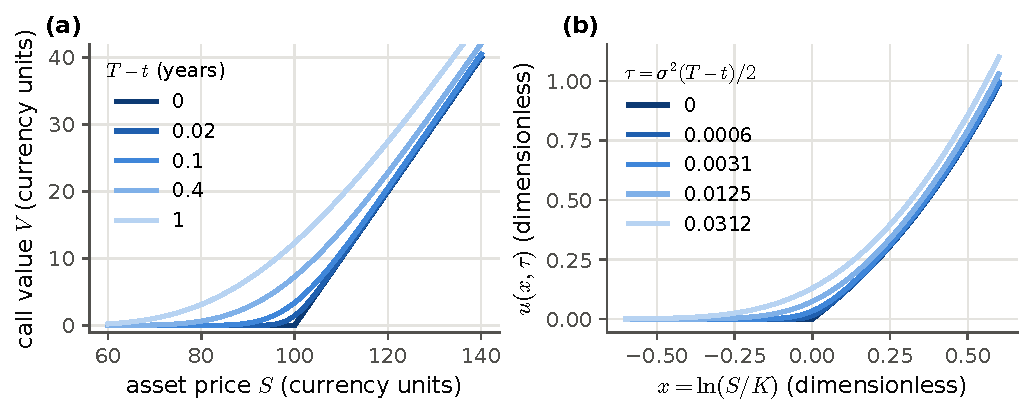
\includegraphics[width=\linewidth]{../figures/fig_smoothing.pdf}
  \caption{(a) Call value $V(S,t)$ for several times to expiry $T-t$; at $T-t=0$ it is the
  payoff~\eqref{eq:payoff}. (b) The same functions as solutions $u(x,\tau)$ of the heat equation
  (\cref{sec:reduction}): a kinked initial temperature profile diffusing along a rod.}
  \label{fig:smoothing}
\end{figure}

%=====================================================================
\section{The Black--Scholes model}\label{sec:model}

The share price follows geometric Brownian motion, $\dd S=\mu S\dd t+\sigma S\dd W$,
with drift $\mu$, volatility $\sigma>0$ and Brownian motion $W$; money in the bank grows at the
constant rate $r$. For a smooth function $V(S,t)$, Itô's lemma (taken as given) states
\begin{equation}\label{eq:ito}
  \dd V=\Big(V_t+\mu S V_S+\tfrac12\sigma^2S^2V_{SS}\Big)\dd t+\sigma S V_S\dd W .
\end{equation}

\paragraph{Delta hedging.} Hold one option and sell $\Delta$ shares: $\Pi=V-\Delta S$. Over $\dd t$,
\[
  \dd\Pi=\dd V-\Delta\dd S=\Big(V_t+\mu SV_S+\tfrac12\sigma^2S^2V_{SS}-\mu\Delta S\Big)\dd t
  +\sigma S\,(V_S-\Delta)\dd W .
\]
Choosing $\Delta=V_S$ removes the random term, and with it the unknown drift $\mu$.
A riskless portfolio must earn the bank rate, otherwise there is an arbitrage, so
$\dd\Pi=r\Pi\dd t=r(V-SV_S)\dd t$. Equating the two expressions for $\dd\Pi$ gives
\begin{equation}\label{eq:bs}
  \boxed{V_t+\tfrac12\sigma^2S^2V_{SS}+rSV_S-rV=0,\qquad S>0,\ t<T,}
\end{equation}
with terminal condition~\eqref{eq:payoff}. The boundary behaviour is
$V(0,t)=0$ (a worthless share stays worthless) and $V(S,t)\sim S-Ke^{-r(T-t)}$ as $S\to\infty$
(the option is then almost surely exercised).

%=====================================================================
\section{Classification and canonical form}\label{sec:classification}

A linear second-order equation in two variables $(X,Y)$,
\[
  A\,w_{XX}+2B\,w_{XY}+C\,w_{YY}+\text{(lower order)}=0,
\]
is \emph{hyperbolic}, \emph{parabolic} or \emph{elliptic} at a point when $B^2-AC$ is positive, zero or
negative there~\cite{myintu,mcowen}. The type is unchanged by smooth invertible changes of variables,
and the characteristic curves solve $A\,\dd Y^2-2B\,\dd X\dd Y+C\,\dd X^2=0$.

For~\eqref{eq:bs} take $(X,Y)=(S,t)$. The principal part is $\tfrac12\sigma^2S^2V_{SS}$, so
\[
  A=\tfrac12\sigma^2S^2,\qquad B=0,\qquad C=0,\qquad B^2-AC=0 .
\]
The equation is \textbf{parabolic} for every $S>0$. The characteristics satisfy $A\,\dd t^2=0$, i.e.\
they are the lines $t=\text{const}$, as for the heat equation. At $S=0$ the whole principal part
vanishes ($A=B=C=0$): the equation \textbf{degenerates} to $V_t-rV=0$, an ODE along the line $S=0$.
For the call this ODE with $V(0,T)=0$ gives $V(0,t)=0$, so the boundary value at $S=0$ is forced by
the equation itself.

\paragraph{Direction of time.} The coefficient of $V_t$ has the same sign as that of $V_{SS}$, which
for the heat equation $u_\tau=u_{xx}$ corresponds to $\tau=T-t$, time running \emph{backwards}.
Hence~\eqref{eq:bs} is a \emph{terminal}-value problem, well posed when solved from $t=T$ backwards.
Solving it forwards in $t$ is the backward heat equation, which is ill posed in the sense of Hadamard:
on $(0,\pi)$ with zero boundary values, the problem $w_t=-w_{xx}$, $w(x,0)=\tfrac1n\sin nx$, has the solution
\begin{equation}\label{eq:hadamard}
  w_n(x,t)=\tfrac1n e^{+n^2t}\sin nx .
\end{equation}
The data tend to zero uniformly as $n\to\infty$, while at any $t>0$ the solution grows without bound
(for $n=20$ the data have size $\hadTwentyData$, and at $t=0.1$ the solution is $\hadTwentySol$).
There is no continuous dependence on the data. \Cref{sec:limits} demonstrates this numerically.

\paragraph{Canonical form.} For parabolic equations the canonical form has a single second
derivative~\cite{myintu,mcowen}. Equation~\eqref{eq:bs} already has this property but with a
variable coefficient $\tfrac12\sigma^2S^2$. The substitution $x=\ln S$ of the next section makes the
coefficient constant, and two further steps remove the lower-order terms entirely.

%=====================================================================
\section{Reduction to the heat equation}\label{sec:reduction}

The reduction below is the classical one~\cite{wilmott}.


\begin{proposition}\label{prop:reduction}
Let $k=2r/\sigma^2$, $\alpha=-\tfrac12(k-1)$, $\beta=-\tfrac14(k+1)^2$, and set
\[
  S=Ke^x,\qquad t=T-\frac{2\tau}{\sigma^2},\qquad V(S,t)=K\,e^{\alpha x+\beta\tau}\,u(x,\tau).
\]
Then $V$ solves~\eqref{eq:bs} with~\eqref{eq:payoff} if and only if
\begin{equation}\label{eq:heativp}
  u_\tau=u_{xx},\quad x\in\mathbb R,\ \tau>0,\qquad
  u(x,0)=u_0(x):=\max\!\big(e^{\frac{k+1}{2}x}-e^{\frac{k-1}{2}x},0\big).
\end{equation}
\end{proposition}

\begin{proof}
\emph{Step 1 (dimensionless variables).} Write $V=Kv(x,\tau)$. By the chain rule,
$\partial_S=\frac1S\partial_x$, so $SV_S=Kv_x$ and $S^2V_{SS}=K(v_{xx}-v_x)$ (differentiate
$SV_S=Kv_x$ once more: $S(SV_S)_S=S^2V_{SS}+SV_S=Kv_{xx}$). Also $\partial_t=-\frac{\sigma^2}{2}\partial_\tau$,
so $V_t=-\frac{\sigma^2}{2}Kv_\tau$. Substituting into~\eqref{eq:bs},
\[
  -\tfrac{\sigma^2}{2}v_\tau+\tfrac{\sigma^2}{2}(v_{xx}-v_x)+rv_x-rv=0 .
\]
Dividing by $\sigma^2/2$ gives
\begin{equation}\label{eq:step1}
  v_\tau=v_{xx}+(k-1)v_x-kv .
\end{equation}
The terminal time $t=T$ becomes $\tau=0$, and $V(S,T)=\max(S-K,0)$ becomes $v(x,0)=\max(e^x-1,0)$.
Only one parameter, $k$, remains ($k=\kval$ for our data).

\emph{Step 2 (removing $v_x$ and $v$).} Put $v=e^{\alpha x+\beta\tau}u$ and write $E=e^{\alpha x+\beta\tau}$. Then
\[
  v_\tau=E(\beta u+u_\tau),\qquad v_x=E(\alpha u+u_x),\qquad v_{xx}=E(\alpha^2u+2\alpha u_x+u_{xx}).
\]
Substituting into~\eqref{eq:step1} and dividing by $E>0$,
\[
  u_\tau=u_{xx}+\big(2\alpha+k-1\big)u_x+\big(\alpha^2+(k-1)\alpha-k-\beta\big)u .
\]
The $u_x$ coefficient vanishes for $\alpha=-\frac{k-1}{2}$. With this $\alpha$,
$\alpha^2+(k-1)\alpha-k=\frac{(k-1)^2}{4}-\frac{(k-1)^2}{2}-k=-\frac{(k+1)^2}{4}$, so the $u$
coefficient vanishes for $\beta=-\frac{(k+1)^2}{4}$. This gives $u_\tau=u_{xx}$.
For the initial condition,
$u(x,0)=e^{-\alpha x}v(x,0)=e^{\frac{k-1}{2}x}\max(e^x-1,0)=\max\big(e^{\frac{k+1}{2}x}-e^{\frac{k-1}{2}x},0\big)$.
Every step is invertible, which gives the converse.
\end{proof}

For our data $\alpha=\alphaval$ and $\beta=\betaval$, and one year to expiry corresponds to
$\tau=\sigma^2T/2=\taufinal$. The boundary conditions transform to $u\to0$ as $x\to-\infty$ and
$u\sim(e^x-e^{-k\tau})e^{-\alpha x-\beta\tau}$ as $x\to\infty$, which grows only like $e^{c|x|}$.
The test suite checks numerically that $u$, computed from the Black--Scholes price, satisfies
$u_\tau=u_{xx}$ (relative finite-difference residual below $10^{-4}$).

%=====================================================================
\section{The heat equation}\label{sec:heat}

We follow the course notes~\cite{classnotes}. In their notation, $t$ is our $\tau$, the diffusivity is
$a^2=k=1$ and the initial data are $g=u_0$.

\paragraph{Separation of variables.} Substituting $u=X(x)T(\tau)$ into $u_\tau=u_{xx}$ gives $XT'=X''T$, and
dividing by $XT$,
\[
  \frac{T'}{T}=\frac{X''}{X}=-\mu^2 .
\]
The left side depends only on $\tau$ and the right only on $x$, so both equal a constant. The constant cannot be
positive: $\kappa^2>0$ would give $X=e^{\pm\kappa x}$, unbounded in $x$. Hence
\[
  T'+\mu^2T=0\ \Rightarrow\ T=Ce^{-\mu^2\tau},\qquad
  X''+\mu^2X=0\ \Rightarrow\ X=A\cos\mu x+B\sin\mu x ,
\]
and higher frequencies $\mu$ decay faster. On an interval $[-l,l]$ boundary conditions would select the
discrete frequencies $n\pi/l$, spaced $\pi/l$ apart, and the solution would be a Fourier series. On $\mathbb R$
there are no boundary conditions, every $\mu\ge0$ is admissible, and as $l\to\infty$ the sum becomes an integral:
\[
  u(x,\tau)=\int_0^\infty e^{-\mu^2\tau}\big(A(\mu)\cos\mu x+B(\mu)\sin\mu x\big)\dd\mu .
\]

\paragraph{The Fourier integral.} At $\tau=0$ the exponential is $1$, so the initial condition asks for $u_0$ as a
Fourier integral, and $A,B$ are the continuous analogues of the Fourier coefficients:
\[
  A(\mu)=\frac1\pi\int_{\mathbb R}u_0(y)\cos\mu y\dd y,\qquad B(\mu)=\frac1\pi\int_{\mathbb R}u_0(y)\sin\mu y\dd y .
\]
Substituting, using $\cos\mu y\cos\mu x+\sin\mu y\sin\mu x=\cos\mu(y-x)$, and exchanging the order of
integration (allowed for $\tau>0$ because of the decaying factor $e^{-\mu^2\tau}$),
\[
  u(x,\tau)=\frac1\pi\int_{\mathbb R}u_0(y)\,I\dd y,\qquad
  I=\int_0^\infty e^{-\mu^2\tau}\cos\mu(y-x)\dd\mu .
\]
The inner integral $I$ does not involve $u_0$. With $z=\mu\sqrt\tau$ and $\eta=(y-x)/\sqrt\tau$,
\[
  I=\frac{1}{\sqrt\tau}K(\eta),\qquad K(\eta)=\int_0^\infty e^{-z^2}\cos\eta z\dd z .
\]
Instead of computing $K$ directly we find an ODE for it. Differentiating under the integral and integrating by
parts with $ze^{-z^2}=-\frac12\frac{\dd}{\dd z}e^{-z^2}$,
\[
  K'(\eta)=-\int_0^\infty ze^{-z^2}\sin\eta z\dd z
  =\Big[\tfrac12e^{-z^2}\sin\eta z\Big]_0^\infty-\frac\eta2\int_0^\infty e^{-z^2}\cos\eta z\dd z=-\frac\eta2K(\eta).
\]
So $K=Ce^{-\eta^2/4}$, and $K(0)=\int_0^\infty e^{-z^2}\dd z=\frac{\sqrt\pi}{2}$ fixes $C$. Then
$I=\frac12\sqrt{\pi/\tau}\,e^{-(y-x)^2/(4\tau)}$, and multiplying by $\frac1\pi$ gives the Fourier--Poisson integral
\begin{equation}\label{eq:conv}
  u(x,\tau)=\int_{\mathbb R}\Phi(x-y,\tau)\,u_0(y)\dd y,\qquad
  \Phi(x,\tau)=\frac{1}{\sqrt{4\pi\tau}}e^{-x^2/(4\tau)}\quad(\tau>0).
\end{equation}
Our $u_0$ is not integrable, so this derivation is formal; \cref{thm:kernel} verifies the result directly.

\paragraph{Second derivation: scaling.} If $u$ solves $u_\tau=u_{xx}$, so does $\lambda u(\lambda x,\lambda^2\tau)$ for every
$\lambda>0$: the time derivative and the two space derivatives each produce a factor $\lambda^2$. The quotient
$x^2/\tau$ is unchanged by this scaling, so we look for $u=w(\tau)\,v(z)$ with $z=x^2/\tau$. Then
\[
  u_\tau=w'v-wv'\frac{x^2}{\tau^2},\qquad u_x=wv'\frac{2x}{\tau},\qquad
  u_{xx}=w\Big(4v''\frac{x^2}{\tau^2}+2v'\frac1\tau\Big),
\]
and $u_\tau=u_{xx}$ becomes
\[
  w'v=w\Big[(4v''+v')\frac{x^2}{\tau^2}+\frac{2v'}{\tau}\Big].
\]
Choose $v$ so that the bracket vanishes: $4v''+v'=0$ gives $v=e^{-z/4}$. The remaining terms give
$w'v=2wv'/\tau=-wv/(2\tau)$, i.e.\ $w'=-w/(2\tau)$ and $w=\tau^{-1/2}$. The amplitude decays like $\tau^{-1/2}$
while the profile spreads over a width of order $\sqrt\tau$, as conservation of heat requires. Finally, choosing
$C$ so that $\int_{\mathbb R}C\tau^{-1/2}e^{-x^2/(4\tau)}\dd x=C\sqrt{4\pi}=1$ gives the fundamental solution
\[
  \Phi(x,\tau)=\begin{cases}\dfrac{1}{\sqrt{4\pi\tau}}e^{-x^2/(4\tau)}, & \tau>0,\\[4pt] 0, & \tau<0,\end{cases}
\]
which is singular at $(0,0)$ and agrees with~\eqref{eq:conv}.

\paragraph{Properties of $\Phi$.}
\begin{enumerate}
  \item[(i)] $\Phi>0$ and $\Phi(x-y,\tau)=\Phi(y-x,\tau)$. If $g\ge0$ is not identically zero, then
    $\Phi*g>0$ everywhere for every $\tau>0$: heat spreads with infinite speed.
  \item[(ii)] $\Phi\in C^\infty$ for $\tau>0$.
  \item[(iii)] $(\partial_\tau-\partial_{xx})\Phi(x-y,\tau)=0$ for every $y$, since
    $\Phi_\tau=\Phi_{xx}=\Phi\big(\frac{x^2}{4\tau^2}-\frac1{2\tau}\big)$ (with $\Phi_x=-\frac{x}{2\tau}\Phi$).
  \item[(iv)] $\int_{\mathbb R}\Phi(x-y,\tau)\dd y=1$, by $y=x+2\sqrt\tau z$ and $\int e^{-z^2}\dd z=\sqrt\pi$. With (i),
    $u=\Phi*g$ is a weighted average of $g$, so $\inf g\le u\le\sup g$.
  \item[(v)] Derivatives and integrals (superpositions) of $\Phi$ are again solutions.
\end{enumerate}
As $\tau\to0^+$, $\Phi(0,\tau)\to\infty$ while $\Phi(x,\tau)\to0$ for $x\neq0$: all the heat concentrates at the
origin, and $\Phi$ is the temperature produced by a unit of heat released at $x=0$ at time $0$.

\begin{theorem}[Initial-value problem~\cite{classnotes,evans}]\label{thm:kernel}
Let $u_0$ be continuous with $|u_0(y)|\le Me^{c|y|}$. Then $u$ defined by~\eqref{eq:conv} is $C^\infty$ for $\tau>0$,
solves $u_\tau=u_{xx}$, and $u(x,\tau)\to u_0(x_0)$ as $(x,\tau)\to(x_0,0^+)$.
\end{theorem}

\begin{proof}
The notes treat bounded $u_0$; the same argument works here because the Gaussian decay of $\Phi$ dominates
$e^{c|y|}$. \emph{Smoothness and the PDE:} for $x$ in a compact set and $\tau$ in a compact subset of $(0,\infty)$,
the $x$- and $\tau$-derivatives of $\Phi(x-y,\tau)u_0(y)$ are bounded by an integrable function of $y$. So we may
differentiate under the integral, and (ii), (iii) give $u\in C^\infty$ with $u_\tau-u_{xx}=0$.
\emph{Initial value:} fix $x_0$ and $\varepsilon>0$, and choose $\delta$ with $|u_0(y)-u_0(x_0)|<\varepsilon$ for
$|y-x_0|<\delta$. By (iv),
\[
  |u(x,\tau)-u_0(x_0)|\le\int_{|y-x_0|<\delta}\Phi\,|u_0(y)-u_0(x_0)|\dd y
  +\int_{|y-x_0|\ge\delta}\Phi\,|u_0(y)-u_0(x_0)|\dd y=:I+J,
\]
and $I\le\varepsilon$ by (i), (iv). If $|x-x_0|<\delta/2$ and $|y-x_0|\ge\delta$, then $|x-y|\ge\frac12|y-x_0|$, so
$J\le(4\pi\tau)^{-1/2}\int_{|y-x_0|\ge\delta}e^{-|y-x_0|^2/(16\tau)}\big(|u_0(y)|+|u_0(x_0)|\big)\dd y\to0$ as $\tau\to0^+$.
Hence $|u(x,\tau)-u_0(x_0)|\le2\varepsilon$ for $(x,\tau)$ close enough to $(x_0,0)$.
\end{proof}

\paragraph{Smoothing.} \Cref{thm:kernel} explains \cref{fig:smoothing}: the kinked payoff becomes
$C^\infty$ at every $\tau>0$. By (i), information spreads at infinite speed (any $\tau>0$ sees all of $u_0$). In
financial terms, every possible future share price affects today's value.

\paragraph{Maximum principle and uniqueness.} Let $\Omega=(a,b)$, let $\Omega_T=\Omega\times(0,T]$ be the parabolic
cylinder, and let $\Gamma_T=\overline{\Omega_T}\setminus\Omega_T$ be its parabolic boundary (bottom and sides).

\begin{theorem}[Weak maximum principle~\cite{classnotes,evans,nandakumaran}]\label{thm:maxprinciple}
If $u\in C^2_1(\Omega_T)\cap C(\overline{\Omega_T})$ solves $u_\tau=u_{xx}$ in $\Omega_T$, then
$\max_{\overline{\Omega_T}}u=\max_{\Gamma_T}u$.
\end{theorem}
The hottest point is attained initially or on the walls; a hot spot cannot appear spontaneously in the interior
or at a later time. Applying the theorem to $-u$ gives the same statement for the minimum. The notes also state
the \emph{strong} form: if $\Omega$ is connected and the maximum is attained at some $(x_0,\tau_0)\in\Omega_T$, then
$u$ is constant on $\Omega_{\tau_0}$. Its proof needs a mean-value property and is not given here.

\begin{proof}
For $\varepsilon>0$ let $u^\varepsilon=u-\varepsilon\tau$, so $u^\varepsilon_\tau-u^\varepsilon_{xx}=-\varepsilon<0$. Suppose
$u^\varepsilon$ attains its maximum over $\overline{\Omega_T}$ at $(x_0,\tau_0)\in\Omega_T$. Then $u^\varepsilon_{xx}\le0$,
and $u^\varepsilon_\tau=0$ if $\tau_0<T$ or $u^\varepsilon_\tau\ge0$ if $\tau_0=T$. Either way
$u^\varepsilon_\tau-u^\varepsilon_{xx}\ge0$, a contradiction. Hence
$\max_{\overline{\Omega_T}}u\le\max_{\overline{\Omega_T}}u^\varepsilon+\varepsilon T=\max_{\Gamma_T}u^\varepsilon+\varepsilon T\le\max_{\Gamma_T}u+\varepsilon T$.
Let $\varepsilon\to0$; the reverse inequality is trivial since $\Gamma_T\subset\overline{\Omega_T}$.
\end{proof}

\begin{theorem}[Uniqueness on a bounded interval]\label{thm:unique}
The problem $u_\tau=u_{xx}$ in $\Omega_T$ with $u$ prescribed on $\Gamma_T$ has at most one solution in
$C^2_1(\Omega_T)\cap C(\overline{\Omega_T})$.
\end{theorem}

\begin{proof}
The difference $w$ of two solutions solves the heat equation with $w=0$ on $\Gamma_T$. \Cref{thm:maxprinciple}
applied to $w$ and to $-w$ gives $\max w=0=\min w$.
\emph{Second proof (energy method).} Let $E(\tau)=\int_\Omega w^2(x,\tau)\dd x$. Then $E\ge0$, and $E(0)=0$
because the bottom of the cylinder is part of $\Gamma_T$. Differentiating under the integral, using the equation
and integrating by parts,
\[
  E'(\tau)=2\int_\Omega ww_\tau\dd x=2\int_\Omega ww_{xx}\dd x
  =-2\int_\Omega w_x^2\dd x+2\big[ww_x\big]_{x=a}^{x=b}=-2\int_\Omega w_x^2\dd x\le0 ,
\]
where the boundary term vanishes because $w=0$ on the sides of the cylinder. So $E$ is non-increasing,
$0\le E(\tau)\le E(0)=0$, and $E\equiv0$. A continuous function whose square has zero integral vanishes, so
$w\equiv0$.
\end{proof}

\begin{theorem}[Maximum principle on $\mathbb R$~\cite{classnotes}]\label{thm:maxline}
Suppose $u\in C^2_1(\mathbb R\times(0,T])\cap C(\mathbb R\times[0,T])$ solves $u_\tau=u_{xx}$ with $u(x,0)=u_0(x)$, and
satisfies the growth estimate $u(x,\tau)\le Ae^{ax^2}$ for constants $A,a>0$. Then
$\sup_{\mathbb R\times[0,T]}u=\sup_{\mathbb R}u_0$.
\end{theorem}
On the whole line there are no walls, so the parabolic boundary is just the initial line. Applied to $\pm w$, the
theorem gives uniqueness within the growth class. Without some growth condition uniqueness fails (Tychonoff's
nonzero solution with zero data). We state this without proof, as the notes do. Our $u$ grows only like
$e^{c|x|}$, so the solution of~\eqref{eq:heativp}, and hence the Black--Scholes price, is unique in this class.

%=====================================================================
\section{The Black--Scholes formula}\label{sec:formula}

\begin{theorem}[Black--Scholes~\cite{blackscholes}]\label{thm:bs}
With $\N(z)=(2\pi)^{-1/2}\int_{-\infty}^z e^{-y^2/2}\dd y$,
\[
  V(S,t)=S\,\N(d_1)-Ke^{-r(T-t)}\N(d_2),\qquad
  d_{1,2}=\frac{\ln(S/K)+(r\pm\frac12\sigma^2)(T-t)}{\sigma\sqrt{T-t}} .
\]
\end{theorem}

\begin{proof}
Since $u_0=0$ for $s<0$, \eqref{eq:conv} splits as $u=I_+-I_-$, where
\[
  I_\pm=\frac{1}{\sqrt{4\pi\tau}}\int_0^\infty e^{\frac{k\pm1}{2}s}\,e^{-(x-s)^2/(4\tau)}\dd s .
\]
Substitute $s=x+\sqrt{2\tau}\,y$, so $\dd s=\sqrt{2\tau}\dd y$, $(x-s)^2/(4\tau)=y^2/2$, and $s>0$
becomes $y>-x/\sqrt{2\tau}$:
\[
  I_\pm=\frac{e^{\frac{k\pm1}{2}x}}{\sqrt{2\pi}}\int_{-x/\sqrt{2\tau}}^{\infty}
        e^{-\frac12y^2+\frac{k\pm1}{2}\sqrt{2\tau}\,y}\dd y .
\]
Completing the square with $m_\pm=\frac{k\pm1}{2}\sqrt{2\tau}$ gives
$-\frac12y^2+m_\pm y=-\frac12(y-m_\pm)^2+\frac12m_\pm^2$, with $\frac12m_\pm^2=\frac{(k\pm1)^2}{4}\tau$. With $z=y-m_\pm$,
\[
  I_\pm=e^{\frac{k\pm1}{2}x+\frac{(k\pm1)^2}{4}\tau}\,\frac{1}{\sqrt{2\pi}}\int_{-x/\sqrt{2\tau}-m_\pm}^{\infty}e^{-z^2/2}\dd z
       =e^{\frac{k\pm1}{2}x+\frac{(k\pm1)^2}{4}\tau}\,\N(d_\pm),
\]
with $d_\pm=\frac{x}{\sqrt{2\tau}}+\frac{k\pm1}{2}\sqrt{2\tau}$, using the symmetry of the Gaussian. Now return to
$V=Ke^{\alpha x+\beta\tau}u$. For $I_+$, $\alpha+\frac{k+1}{2}=1$ and $\beta+\frac{(k+1)^2}{4}=0$, so the
prefactor is $Ke^x=S$. For $I_-$, $\alpha+\frac{k-1}{2}=0$ and
$\beta+\frac{(k-1)^2}{4}=\frac{(k-1)^2-(k+1)^2}{4}=-k$, so the prefactor is $Ke^{-k\tau}=Ke^{-r(T-t)}$
because $k\tau=\frac{2r}{\sigma^2}\cdot\frac{\sigma^2(T-t)}{2}$. Finally $\sqrt{2\tau}=\sigma\sqrt{T-t}$ and $x=\ln(S/K)$ give
$d_+=\frac{\ln(S/K)}{\sigma\sqrt{T-t}}+\big(\frac{r}{\sigma^2}+\frac12\big)\sigma\sqrt{T-t}=d_1$, and likewise $d_-=d_2$.
\end{proof}

\paragraph{Checks.} (i) \emph{Put--call parity.} The put satisfies the same PDE with payoff $\max(K-S,0)$,
and $C-P$ solves~\eqref{eq:bs} with payoff $S-K$, whose solution is $S-Ke^{-r(T-t)}$. Numerically
$|C-P-(S-Ke^{-r(T-t)})|\le\parityGap$ on $S\in[20,300]$.
(ii) \emph{Limits.} As $S\to0$, $d_{1,2}\to-\infty$ and $V\to0$; as $S\to\infty$, $\N(d_{1,2})\to1$ and
$V\sim S-Ke^{-r(T-t)}$; as $t\to T$, $d_{1,2}\to\pm\infty$ according to the sign of $\ln(S/K)$, so $V\to\max(S-K,0)$.

%=====================================================================
\section{Separation of variables: the double-barrier option}\label{sec:barrier}

A double-barrier knock-out call pays $\max(S-K,0)$ at $T$ unless the share price touches $B_1$ or $B_2$
($B_1<K<B_2$) before expiry, in which case it becomes worthless. Its value satisfies~\eqref{eq:bs} on
$B_1<S<B_2$ with $V(B_1,t)=V(B_2,t)=0$. Because $V=Ke^{\alpha x+\beta\tau}u$ and the exponential is
positive, the reduction of \cref{prop:reduction} gives
\begin{equation}\label{eq:barrierpde}
  u_\tau=u_{xx},\ a<x<b,\qquad u(a,\tau)=u(b,\tau)=0,\qquad u(x,0)=u_0(x),
\end{equation}
with $a=\ln(B_1/K)=\barA$, $b=\ln(B_2/K)=\barB$, $\ell=b-a=\barEll$.

\paragraph{Separation.} Look for $u=X(x)\Theta(\tau)\not\equiv0$. Then $X\Theta'=X''\Theta$, and
$\Theta'/\Theta=X''/X$ must be a constant $-\lambda$:
\[
  X''+\lambda X=0,\qquad X(a)=X(b)=0,\qquad \Theta'=-\lambda\Theta .
\]
\emph{Case $\lambda<0$}, $\lambda=-\mu^2$: $X=Ae^{\mu(x-a)}+Be^{-\mu(x-a)}$. Then $X(a)=0$ gives $B=-A$, and
$X(b)=2A\sinh(\mu\ell)=0$ gives $A=0$. \emph{Case $\lambda=0$}: $X=A+B(x-a)$, and the boundary
conditions give $A=B=0$. \emph{Case $\lambda>0$}: $X=A\cos(\sqrt\lambda(x-a))+B\sin(\sqrt\lambda(x-a))$.
Then $X(a)=0$ gives $A=0$, and $X(b)=B\sin(\sqrt\lambda\,\ell)=0$ with $B\neq0$ requires
$\sqrt\lambda\,\ell=n\pi$. So the eigenpairs are
\[
  \lambda_n=\Big(\frac{n\pi}{\ell}\Big)^2,\qquad X_n(x)=\sin\frac{n\pi(x-a)}{\ell},\qquad
  \Theta_n=e^{-\lambda_n\tau},\qquad n=1,2,\dots
\]
Superposing and using the orthogonality $\int_a^bX_mX_n\dd x=\frac{\ell}{2}\delta_{mn}$ to match $u_0$:
\begin{equation}\label{eq:series}
  u(x,\tau)=\sum_{n=1}^\infty c_n\sin\frac{n\pi(x-a)}{\ell}e^{-(n\pi/\ell)^2\tau},\qquad
  c_n=\frac2\ell\int_{\max(a,0)}^{b}u_0(x)\sin\frac{n\pi(x-a)}{\ell}\dd x .
\end{equation}
The lower limit is $\max(a,0)$ because $u_0=0$ for $x<0$. The coefficients are computed by adaptive
quadrature with an oscillatory weight (\texttt{barrier.py}).

\begin{remark}[Uniqueness and a corner]
\Cref{thm:unique} applies to~\eqref{eq:barrierpde} except for one subtlety: $u_0(b)\neq0$ while
$u(b,\tau)=0$, so the data are discontinuous at the corner $(b,0)$ and $u\notin C(\overline{U_T})$.
Uniqueness still holds by the energy method of \cref{thm:unique}, which needs only $w(\cdot,\tau)\to0$ in
$L^2$ rather than continuity at the corner. For the difference $w$ of two solutions,
$\frac{\dd}{\dd\tau}\int_a^bw^2\dd x=-2\int_a^bw_x^2\dd x\le0$ (integrate by parts using $w(a)=w(b)=0$),
and $\int_a^b w^2\dd x\to0$ as $\tau\to0$. Hence $w\equiv0$.
\end{remark}

\paragraph{Convergence of the series.} Since $u_0$ does not vanish at $b$, $c_n=O(1/n)$ and the series
converges slowly at $\tau=0$. For $\tau>0$ the factor $e^{-(n\pi/\ell)^2\tau}$ makes it converge faster
than geometrically. If $N$ terms are needed for an error of order $\varepsilon$, then
$e^{-(N\pi/\ell)^2\tau}\approx\varepsilon$, i.e.\
\[
  N\approx\frac{\ell}{\pi}\sqrt{\frac{\ln(1/\varepsilon)}{\tau}}\ \propto\ (T-t)^{-1/2}.
\]
\Cref{fig:barrier}(b) confirms this. For $10^{-4}$ accuracy in price, \termsLongest{} terms suffice one year
before expiry, but \termsShortest{} are needed one day before. The estimate above gives \termsPredLongest{}
and \termsPredShortest{} respectively. Against a Crank--Nicolson solution of~\eqref{eq:barrierpde}
(2000 intervals, 2000 steps) the series agrees to within $\barDiffMax$ at $T-t\in\{0.1,0.5,1\}$
(\cref{fig:barrier}(a)). At $S=100$ the barrier option costs $\barPriceHundred$, against
$\priceHundred$ for the vanilla call, because paths that would pay the most are knocked out.

\begin{figure}[t]
  \centering
  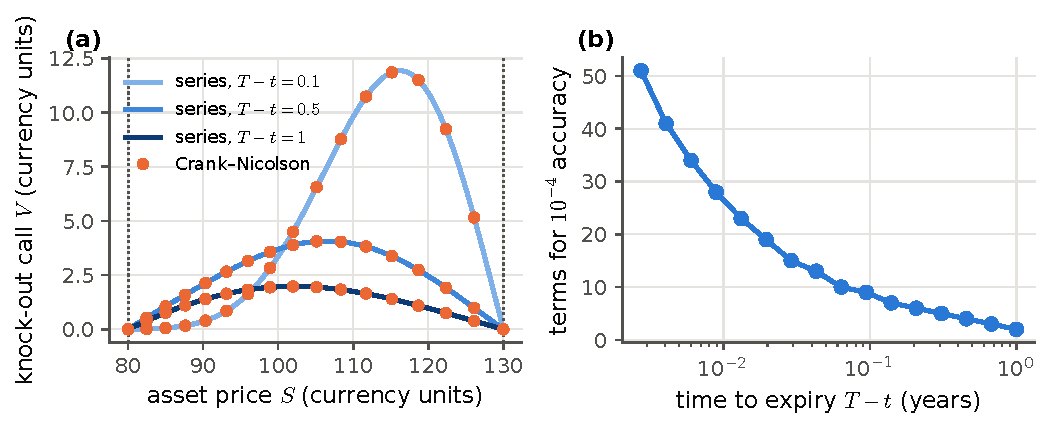
\includegraphics[width=\linewidth]{../figures/fig_barrier.pdf}
  \caption{Double-barrier knock-out call, $B_1=\Bone$, $B_2=\Btwo$. (a) Fourier series (lines) against
  Crank--Nicolson (markers) for three times to expiry. (b) Number of series terms needed for
  $10^{-4}$ accuracy against time to expiry.}
  \label{fig:barrier}
\end{figure}

%=====================================================================
\section{Limitations and conclusion}\label{sec:limits}

\paragraph{Model limitations.} The reduction relies on constant $\sigma$ and $r$. With $\sigma=\sigma(S,t)$ the
coefficients stay variable after the substitution and no closed form exists in general. Dividends add a
term $-qSV_S$, which the same method absorbs; jumps in the share price turn the PDE into a
partial integro-differential equation; early exercise (American options) gives a free-boundary problem.
The barriers here are monitored continuously; in practice they are usually checked daily.

\paragraph{Ill-posedness of forward solving.} The Black--Scholes problem must be solved backwards from
expiry. \Cref{fig:illposed} shows what happens otherwise. We march the heat equation backwards from
$\sin x$ on $(0,\pi)$ with noise of size $\illEps$ (\illModes{} sine modes), multiplying each sine coefficient
by $e^{+n^2t}$ as in~\eqref{eq:hadamard}. After $t=0.0005$ the maximum is $\illMaxNoisyHalfMilli$, after $t=0.001$
it is $\illMaxNoisyOneMilli$, and after $t=0.002$ it is $\illMaxNoisyTwoMilli$, although the exact backward solution
is just $e^{t}\sin x\approx\sin x$. Even without added noise, floating-point rounding errors alone reach
$\illMaxCleanThreeMilli$ by $t=0.003$. This is the numerical face of Hadamard ill-posedness.

\begin{figure}[t]
  \centering
  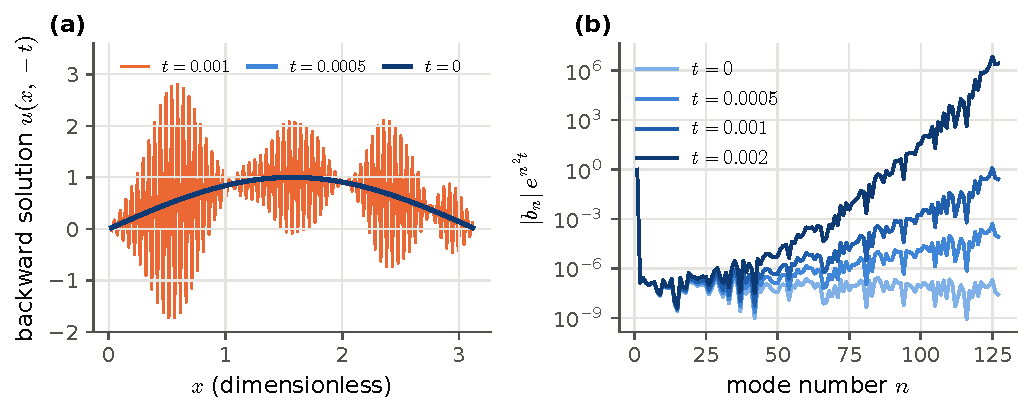
\includegraphics[width=\linewidth]{../figures/fig_illposed.pdf}
  \caption{Backward heat equation from $\sin x$ plus noise of size $\illEps$. (a) The solution after marching
  backwards for time $t$. (b) Size of the sine coefficients $|b_n|e^{n^2t}$: high modes grow like $e^{n^2t}$.}
  \label{fig:illposed}
\end{figure}

\paragraph{Conclusion.} The Black--Scholes equation is a degenerate parabolic terminal-value problem.
After $S=Ke^x$, $t=T-2\tau/\sigma^2$ and $V=Ke^{\alpha x+\beta\tau}u$ it \emph{is} the heat equation. The heat
kernel, obtained from the Fourier integral or from scaling, gives the Black--Scholes formula, and the
maximum principle and the energy method show that it is the only solution in its growth class. Separation
of variables prices a double-barrier option, and its series needs $O((T-t)^{-1/2})$ terms near expiry.

\label{lastbodypage}
\bibliographystyle{plain}
\bibliography{refs}

\end{document}
